\chapter{Informatyka afektywna}
\label{cha:affectiveComputing}

Informatyka afektywna (ang. \textit{affective computing}) jest dziedziną informatyki, w~której obliczenia są powiązane z emocjami, lub bezpośrednio na nie wpływają~\cite{Picard:1997:AC:265013}. Głównym celem informatyki afektywnej jest rozpoznawanie oraz analiza emocji ludzkich, możliwość ich symulacji przez komputer, a także wpływanie na emocje użytkownika poprzez konkretne bodźce. Aby uzyskać taki efekt, informatyka afektywna jest silnie powiązana z dziedzinami takimi jak psychologia, fizjologia, czy kognitywistyka~\cite{affective_computing_review_tao_tieniu}.

\section{Emocje}
Choć do dzisiaj nie ma jednej, uniwersalnej definicji czym są emocje, to środowisko naukowe ciągle przeprowadza badania na tematy powiązane z emocjami. Już w~XIX wieku powstała teoria opracowana niezależnie przez Williama Jamesa oraz Carla Lange'a, w~której emocję zdefiniowano jako interpretację reakcji cielesnej na zaobserwowany bodziec~\cite{Coleman2011}. Obaj badacze przyjęli, że na konkretny czynnik człowiek reaguje najpierw reakcją fizjologiczną, która następnie zostaje przez niego przypisana do wzorca odpowiadającego danej emocji. Dla przykładu, jeśli człowiek znajdzie się w~sytuacji, w~której zobaczy zagrożenie, zaczyna się trząść i~pocić, a jego tętno gwałtownie wzrasta, jego mózg natomiast interpretuje to jako strach.

Teoria Jamesa-Lange'a została zakwestionowana w~latach dwudziestych XX wieku przez dwójkę naukowców, Waltera Cannona i~Phillipa Barda. Zasugerowali oni, że odczuwanie emocji nie jest zależne od reakcji fizjologicznych, a raczej są to reakcje zachodzące jednocześnie jako odpowiedź na dany bodziec~\cite{cannon_1927}. Teoria ta była bezpośrednim zakwestionowaniem badań przeprowadzonych przez Jamesa i~Lange'a. Jej autorzy przeprowadzili badania na kotach, na podstawie których przedstawili, że to wzgórze jest obszarem mózgu odpowiedzialnym za reakcje emocjonalne na doświadczane bodźce. Cannon zauważył, że całkowite odcięcie wszystkich układów od mózgu nie zmienia zachowania emocjonalnego zwierząt, co kłóciło się z teorią Jamesa-Lange'a, według której koty powinny przestać wykazywać jakiekolwiek reakcje emocjonalne.

\begin{figure}[h]
	\centering
	\begin{subfigure}{0.7\textwidth}
		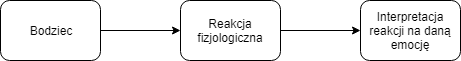
\includegraphics[width=\linewidth]{images/james-lang.png}
		\label{fig:james}
		\caption{Teoria Jamesa-Lange'a, źródło: opracowanie własne na podstawie~\cite{Coleman2011}}
	\end{subfigure}
	\begin{subfigure}{0.7\textwidth}
		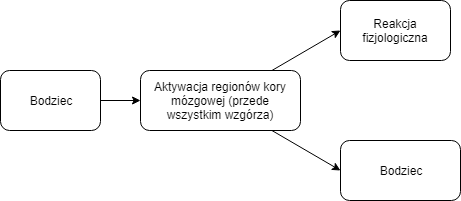
\includegraphics[width=\linewidth]{images/cannon-bard.png}
		\label{fig:canon}
		\caption{Teoria Canona-Barda, źródło: opracowanie własne na podstawie~\cite{cannon_1927}}
	\end{subfigure}
	\caption{Graficzne porównanie teorii emocji Jamesa-Lange'a i Canona-Barda}
\end{figure}

Teoria Jamesa-Lange'a została ponownie podjęta przez Prinza, który przedstawił więcej dowodów na potwierdzenie tej teorii, jednocześnie opisując argumenty pokazujące, że reakcje fizjologiczne nie zawsze są wystarczające, lub w~ogóle niepotrzebne do odczuwania emocji~\cite{Prinz2004-PRIEE-2}. Zwrócił on między innymi uwagę na badania Hohmanna nad pacjentami z urazami rdzenia kręgowego~\cite{Hohmann1966SomeEO}, w~których zauważono efekty zarówno potwierdzające, jak i podające w~wątpliwość teorię Jamesa-Lange'a. Hohmann zauważył, że u osób z urazem można zauważyć redukcję w~odczuwaniu emocji, ale niektóre z nich wciąż były zauważalne. Prinz komentuje to jako zdolność mózgu do przewidzenia reakcji fizjologicznej na dany bodziec, co z kolei będzie skutkować odczuwaniem emocji. Jest to możliwe dzięki wcześniejszym doświadczeniom. Tak jak człowiek, który stracił wzrok, jest w~stanie wyobrazić sobie przedmiot, który kiedyś widział, tak samo mózg potrafi określić jaka reakcja fizjologiczna mogła nastąpić na dany bodziec.

\section{Modele emocji}
Ponieważ emocje są pojęciem abstrakcyjnym, ich pomiar oraz analiza w~informatyce afektywnej nie jest prosta i wymaga przyjętego modelu, który pozwoli na jednoznaczny pomiar emocji. Na przestrzeni lat powstało wiele modeli opisujących emocje, które można podzielić na dwie główne kategorie~\cite{emotion_models_review_2017}:
\begin{itemize}
	\item modele kategoryzowane, w~których określony jest zbiór emocji reprezentowanych przez konkretne oznaczenia
	\item modele wymiarowe, w~których emocje są reprezentowane przy pomocy zbioru miar określających ich własności.
\end{itemize}

\subsection{Modele kategoryzowane}
Do typu modeli kategoryzowanych zaliczają się przede wszystkim modele emocji bazowych. Na przestrzeni lat powstało wiele modeli różniących się od siebie ilością oraz rodzajami emocji. Przykładem może być tutaj model zaproponowany przez Oatley'a i Johnsona-Lairda, w~którym proponują oni pięć podstawowych emocji: gniew, lęk, odraza, radość i smutek~\cite{oatley_theory_of_emotions}. Jednym z popularniejszych modeli emocji bazowych, jest ten przedstawiony przez Ekmana. Razem z Friesenem przeprowadzili badania na plemieniu z Papui Nowej Gwinei. Członkowie plemienia byli w~stanie zidentyfikować sześć emocji: strach, gniew, wstręt, smutek, szczęście i zaskoczenie (rys. \ref{fig:ekman_six_emotions})~\cite{Ekman1971ConstantsAC}. Kilka lat później do tej grupy Ekman dodał pogardę, aby odróżnić ją od wstrętu. 
\begin{figure}[h]
	\centering
	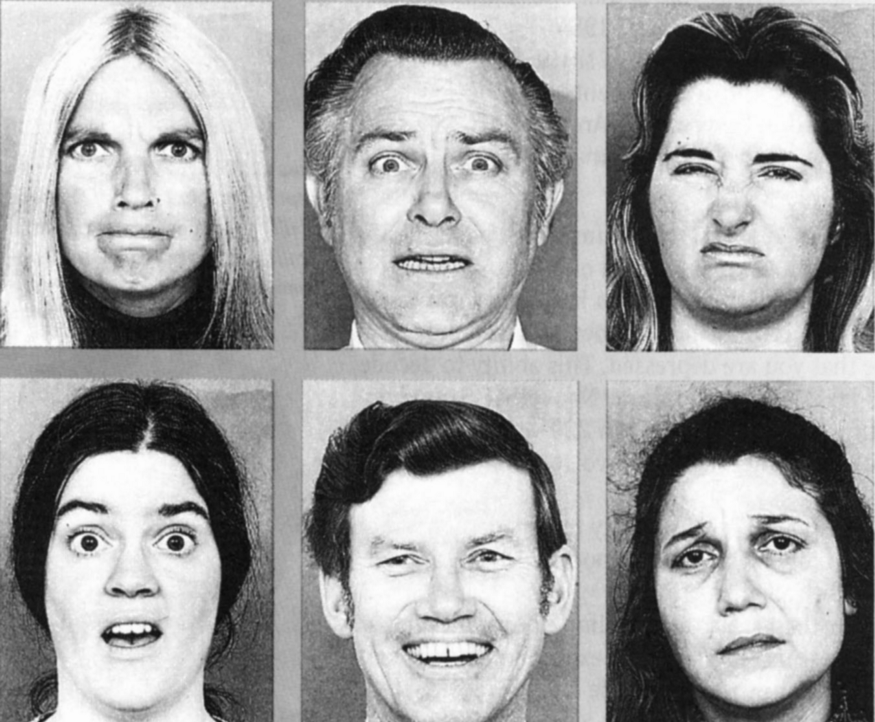
\includegraphics[width=0.6\linewidth]{images/ekman_six_basic_emotions.png}
	\caption{Wyrazy twarzy odpowiadające sześciu emocjom zaproponowanym przez Ekmana, źródło: \cite{Ekman1971ConstantsAC}}
	\label{fig:ekman_six_emotions}
\end{figure}

W modelach kategoryzowanych często nazywanych także modelami dyskretnymi emocje są niezależne od siebie. Ich dużą zaletą jest to, że automatycznie reprezentują ludzkie emocje dzięki łatwym do zrozumienia etykietom. Jednak w~swojej pracy James Russell i Lisa Barret przedstawiają problemy, jakie można napotkać w~tym typie modeli~\cite{russel_barret_core_affect}. Pierwszym są różnice występujące w~nazwach kategorii w~zależności od języka. Każdy ze stanów emocjonalnych może być opisany na różne sposoby w~zależności od języka. Różnice mogą wystąpić nie tylko w~samym tłumaczeniu, ale nawet w~ilości słów opisujących daną emocję. Drugim problemem jest to, że granice pomiędzy danymi kategoriami emocji często są rozmyte. Te same stany emocjonalne można wyrazić za pomocą różnych kategorii w~zależności od różnic kulturowych, środowiskowych czy osobowościowych~\cite{emotion_models_review_2017}. Trzecim przedstawionym problemem jest to, że każda z kategorii emocji, takich jak gniew, czy strach składają się z zestawu uporządkowanych w czasie, powiązanych ze sobą zdarzeń. W związku z tym takie emocje powinno traktować jako złożone procesy, które nie powinny być traktowane jako elementy atomowe.

\subsection{Modele wymiarowe}

Russell w swoich badaniach zauważył jeszcze jeden istotny problem modeli dyskretnych. Ponieważ opisują one stany emocjonalne w sposób jednoznaczny, nie można określić poziomu odczuwania emocji. Jako przykład podaje porównanie strachu w trakcie przejażdżki kolejką górską a sytuacjami zagrażającymi życiu. W przypadku modeli dyskretnych w obu sytuacjach można jedynie określić odczuwanie emocji strachu, pomimo różniących się reakcji fizjologicznych. W ramach swoich badań Russel zaproponował model w kształcie okręgu, składający się z dwóch wymiarów (rys. \ref{fig:circumplex}). Pierwszym z nich jest poziom odczuwania przyjemności w modelu nazwany wartościowością (ang. \textit{valence}). Odzwierciedlał on także pozytywność lub negatywność emocji. Niskie wartości odpowiadają emocjom takim jak smutek, stres, czy odraza, natomiast szczęście lub ekscytacja są opisane przez wysokie wartości wartościowości. Drugim wymiarem jest pobudzenie (ang. \textit{arousal}), które opisuje natężenie danej emocji. Odczucia takiej jak senność, depresja czy zrelaksowanie charakteryzują się niskimi wartościami pobudzenia, natomiast wartościom wysokim odpowiadają emocje takie jak ekscytacja, zaskoczenie, czy złość. Model został przedstawiony w formie koła, na którego brzegach opisane zostały podstawowe emocje. Warto wspomnieć, że nie jest to pierwszy model o strukturze kołowej. Sam Russel, chcąc pokazać uniwersalność swojego modelu, porównuje go między innymi z teoriami zaproponowanymi przez Watsona i Tellegena~\cite{Watson_1985}. Tym, co wyróżniało model Russela, były przeprowadzone badania~\cite{circumplex_model_russel_1980}. Russel wybrał 28 słów reprezentujących konkretne stany afektywne i przy pomocy trzech różnych technik przeskalował je, otrzymując zbliżone wyniki. Aby potwierdzić swoją teorię, przeprowadził eksperyment z grupą 36 osób, która miała przyporządkować wybrane słowa do ośmiu kategorii określających podstawowe stany emocjonalne, a następnie ułożyć te kategorie na modelu kołowym w taki sposób, aby przeciwne emocje znalazły się po przeciwnych stronach koła.

\begin{figure}[h]
	\centering
	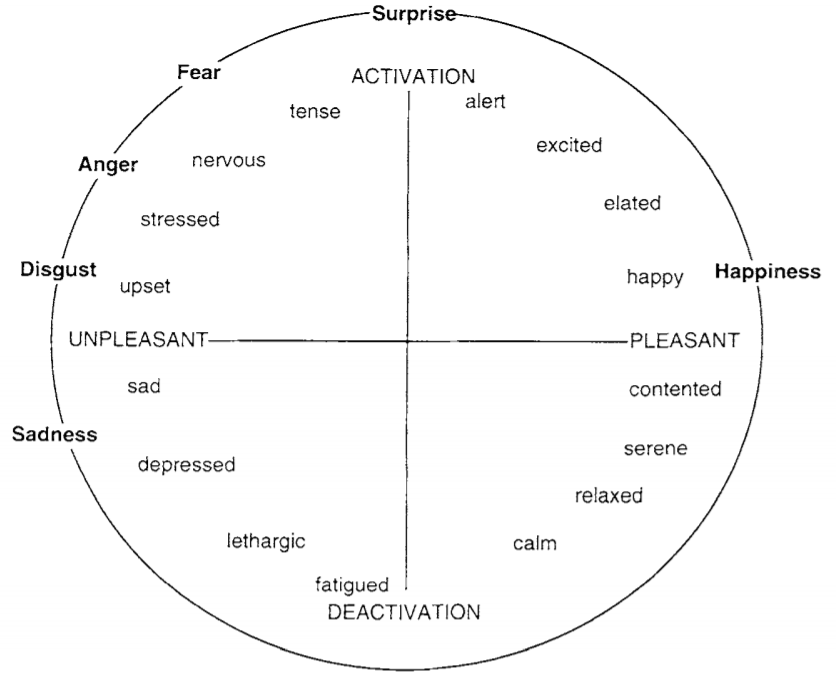
\includegraphics[width=0.6\linewidth]{images/circumplex.png}
	\caption{Model wymiarowy zaproponowany przez Russela, źródło: \cite{russel_barret_core_affect}}
	\label{fig:circumplex}
\end{figure}

Kilka lat później Russel wraz z Anną Weiss oraz Geraldem Mendelsohnem przedstawił propozycję jednopunktowej skali nazwaną Affect Grid, która miała służyć jako sposób szybkiej i prostej do analizy oceny stanów afektywnych wzdłuż wymiarów znanych z modelu Russela, wartościowości oraz pobudzenia~\cite{affect_grid_russel_1989}. Skala jest przedstawiona w formie siatki, gdzie oba wymiary określane są w zakresach od 1 do 9 w sposób ciągły. Początkowo miała ona mieć formę kołową, podobną kołowej struktury modeli emocji, jednak ostatecznie zrezygnowano z niej na rzecz siatki, która była znacznie prostsza do wyjaśnienia badanym osobom. W ramach sprawdzenia, czy przedstawiona skala w poprawny sposób odzwierciedla stany emocjonalne, przeprowadzono badania, w których wykorzystano między innymi słowa wybrane przy wcześniejszych badaniach Russela oraz zbiór zdjęć z wyrazami twarzy odpowiadającymi konkretnym stanom afektywnym. Zadaniem badanych było oznaczenie na skali poziomu wartościowości i pobudzenia, które najlepiej odzwierciedlały dane słowo lub wyraz twarzy. Następnie wyniki porównano z innymi skalami opisującymi poziomy wartościowości i zauważono wysoki procent podobieństwa między nimi. 

\begin{figure}[h]
	\centering
	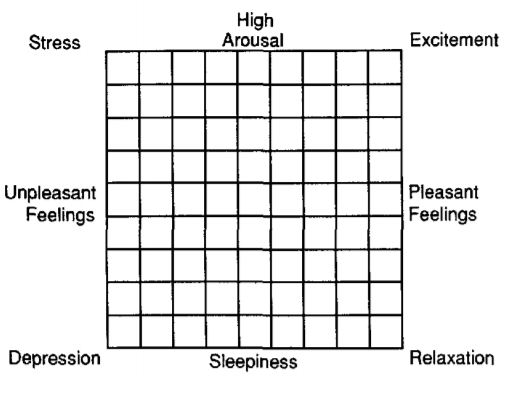
\includegraphics[width=0.5\linewidth]{images/affect_grid.png}
	\caption{Affect Grid, źródło:~\cite{affect_grid_russel_1989}}
	\label{fig:affect_grid}
\end{figure}

Model emocji przedstawiony przez Russela oraz skala opisana w Affect Grid stały się jednymi z bardziej popularnych form przedstawiania emocji w informatyce afektywnej. Ogromną zaletą jest przede wszystkim łatwość przetwarzania danych opartych na dwuwymiarowej skali, które określają dane stany emocjonalne. Skalę tą można zauważyć między innymi w zbiorach danych zawierających powiązania między reakcjami fizjologicznymi a odpowiednimi wartościami wartościowości i pobudzenia~\cite{deap_dataset_2011,amigos_dataset_2017}. 

\section{Pętla afektywna}
\url{https://www.researchgate.net/publication/220962601_Affective_Loop_Experiences_-_What_Are_They/link/0deec530769158251e000000/download}
Co to jest pętla afektywna, jaki jest schemat pętli



\section{Gry z pętlą afektywną}
Jakie mogą być mechaniki (krótko), przykłady takich gier (proste - gry z wyborem wpływającym na rozgrywkę, złożone - Nevermind, Bring to Light)

\url{https://www.researchgate.net/profile/Eva_Hudlicka/ publication/228622615_Affective_computing_for_game_design/links/02bfe50e1936ab5b93000000/Affective-computing-for-game-design.pdf/}

\url{https://www.gamesradar.com/horror-game-nevermind-uses-biometrics-sense-your-fear/}

\url{https://store.steampowered.com/app/636720/Bring_to_Light/}


